% !TEX TS-program = pdflatex
% !TEX encoding = UTF-8 Unicode

% This file is a template using the "beamer" package to create slides for a talk or presentation
% - Giving a talk on some subject.
% - The talk is between 15min and 45min long.
% - Style is ornate.

% MODIFIED by Jonathan Kew, 2008-07-06
% The header comments and encoding in this file were modified for inclusion with TeXworks.
% The content is otherwise unchanged from the original distributed with the beamer package.

\documentclass{beamer}
\setbeamercovered{invisible}



% Copyright 2004 by Till Tantau <tantau@users.sourceforge.net>.
%
% In principle, this file can be redistributed and/or modified under
% the terms of the GNU Public License, version 2.
%
% However, this file is supposed to be a template to be modified
% for your own needs. For this reason, if you use this file as a
% template and not specifically distribute it as part of a another
% package/program, I grant the extra permission to freely copy and
% modify this file as you see fit and even to delete this copyright
% notice. 


\mode<presentation>
{
  \usetheme{Warsaw}
  % or ...

  % or whatever (possibly just delete it)
}


\usepackage[english]{babel}
% or whatever

\usepackage[utf8]{inputenc}
\usepackage{qrcode}
\usepackage{hyperref}
\usepackage{ytableau}
\usepackage{longtable}
% or whatever

\usepackage{times}
\usepackage[T1]{fontenc}
\usepackage{tikz}
% Or whatever. Note that the encoding and the font should match. If T1
% does not look nice, try deleting the line with the fontenc.

%%% MATH RELATED

\title{MATH 180 Strategies of Problem Solving} 
\subtitle
{} % (optional)

\author[W.R. Casper] % (optional, use only with lots of authors)
{W.R. Casper}
% - Use the \inst{?} command only if the authors have different
%   affiliation.

\institute[California State University Fullerton] % (optional, but mostly needed)
{
  Department of Mathematics\\
  California State University Fullerton}
% - Use the \inst command only if there are several affiliations.
% - Keep it simple, no one is interested in your street address.

\subject{Talks}
% This is only inserted into the PDF information catalog. Can be left
% out. 



% If you have a file called "university-logo-filename.xxx", where xxx
% is a graphic format that can be processed by latex or pdflatex,
% resp., then you can add a logo as follows:

% \pgfdeclareimage[height=0.5cm]{university-logo}{university-logo-filename}
% \logo{\pgfuseimage{university-logo}}



% Delete this, if you do not want the table of contents to pop up at
% the beginning of each subsection:
\AtBeginSubsection[]
{
  \begin{frame}<beamer>{Outline}
    \tableofcontents[currentsection,currentsubsection]
  \end{frame}
}


% If you wish to uncover everything in a step-wise fashion, uncomment
% the following command: 

%\beamerdefaultoverlayspecification{<+->}


\begin{document}

\begin{frame}
  \titlepage
\end{frame}

\begin{frame}{Outline}
  \tableofcontents
  % You might wish to add the option [pausesections]
\end{frame}

% Since this a solution template for a generic talk, very little can
% be said about how it should be structured. However, the talk length
% of between 15min and 45min and the theme suggest that you stick to
% the following rules:  

% - Exactly two or three sections (other than the summary).
% - At *most* three subsections per section.
% - Talk about 30s to 2min per frame. So there should be between about
%   15 and 30 frames, all told.

\section{SoPS Lecture 11}

\begin{frame}{Review}
  \begin{block}{Last time}
    \begin{itemize}
\pause
      \item we learned the degree sum formula
      \item we learned Euler's formula for planar graphs
      \item questions about Sprouts
    \end{itemize}
  \end{block}
\end{frame}

\begin{frame}{First-year/Transfer Event}
  \begin{center}
    \qrcode[hyperlink,height=4cm]{https://whenavailable.com/invite/RdQejLJ6uuLgJ5n83xNW}
  \end{center}
\end{frame}

\subsection{Konigsberg bridge problem}

\begin{frame}{Bridges of Konigsberg}
  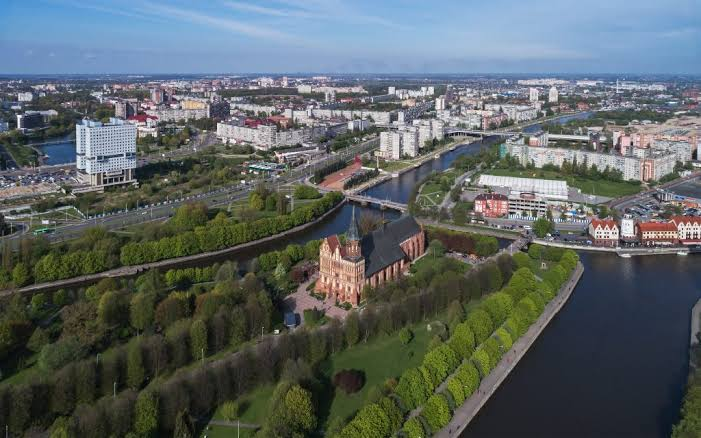
\includegraphics[width=\linewidth]{fig/bridges1}
\end{frame}

\begin{frame}{Bridges of Konigsberg}
  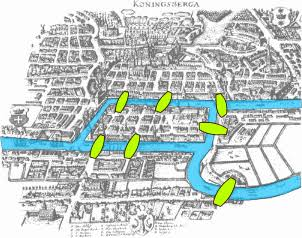
\includegraphics[width=\linewidth]{fig/bridges2}
\end{frame}

\begin{frame}{Bridges of Konigsberg}
  \begin{block}{Problem:}
    Can one find a route which crosses every bridge exactly one time?
  \end{block}
\end{frame}

\begin{frame}{Bridges of Konigsberg}
  \begin{center}
    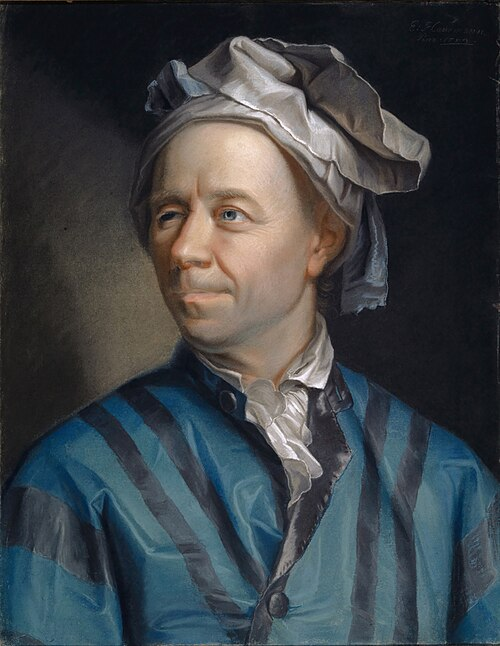
\includegraphics[height=0.6\linewidth]{fig/bridges3}
  \end{center}
\end{frame}

\begin{frame}{Bridges of Konigsberg}
  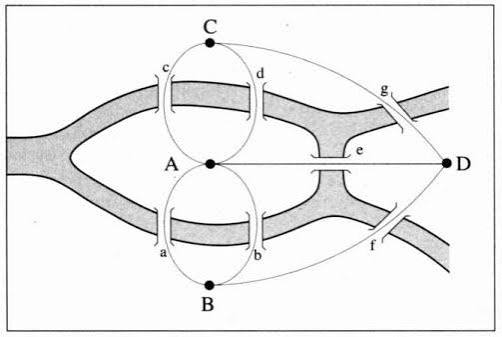
\includegraphics[width=\linewidth]{fig/bridges4}
\end{frame}

\begin{frame}{Eulerian Paths}
  \begin{block}{Defintion}
    An \textbf{Eulerian path} in a graph is a sequence of edges that you can walk along to visit every vertex exactly one time.
  \end{block}
\end{frame}

\begin{frame}{Eulerian Paths}
\pause
  \begin{block}{Theorem:}
    A graph has an Eulerian path if and only if it has less two or less nodes with odd degree.
  \end{block}
\pause
  \begin{block}{Corollary:}
    The Konigsberg bridge problem has no solution!
  \end{block}
\end{frame}

\begin{frame}{Math is creative}
  \begin{itemize}
\pause
    \item Euler's Konigsberg bridge problem.
\pause
    \item $1 + 3 + 5 + 7 + \dots + 2n+1 = $
  \end{itemize}
\end{frame}

\begin{frame}{Creative Konigsberg solution}
  \begin{center}
    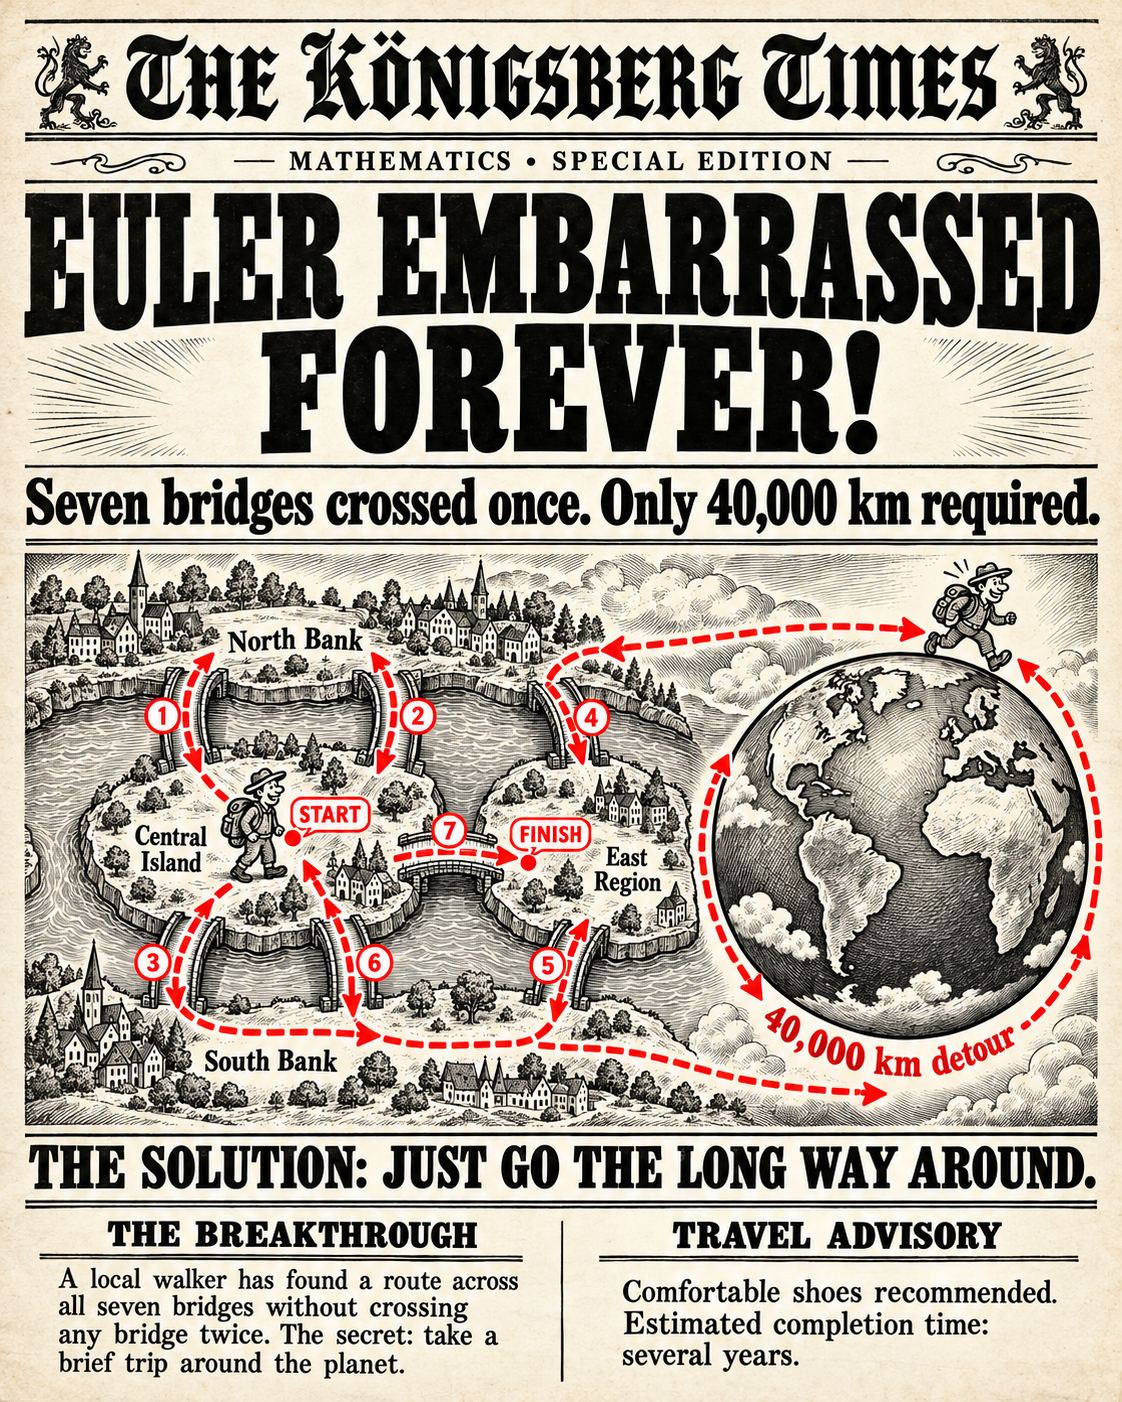
\includegraphics[width=.5\linewidth]{fig/bridges5}
  \end{center}
\end{frame}

\subsection{Math and creativity}

\begin{frame}{Challenge problem}
  \begin{block}{Activity:}
    Color every dot in a \(4\times4\) grid red or blue, avoiding any rectangle with horizontal and vertical sides whose four corners have the same color. Rectangles of every size count.  If you succeed, try \(5\times5\).
  \end{block}
\end{frame}

\begin{frame}{Challenge problem}
  \begin{block}{Discussion:}
    What did you try and what did it reveal?
  \end{block}
\end{frame}

\begin{frame}{Computation vs. Creative Math}
\pause
  \begin{block}{Computation:}
    You're applying a known method.  No creativity needed.
  \end{block}
\pause
  \begin{block}{Creative Math:}
    You're approaching a problem where the way to solve it isn't known.  You have to \textit{get creative}.
  \end{block}
\end{frame}

\begin{frame}{You can always play}
\pause
  Not knowing what to do {\color{red} is fun}!
\pause
  \begin{block}{Remember:}
    You can never really be \textbf{stuck on a problem}.  There's always something more to do/try.
\pause
    Accept the discomfort of not knowing.
  \end{block}
  \begin{itemize}
\pause
    \item make the problem smaller
\pause
    \item try something deliberately unusual
\pause
    \item change the way data is represented
\pause
    \item examine previous failures and why they failed
\pause
    \item play ``what if"
\pause
    \item make a conjecture -- then try to break it
  \end{itemize}
\end{frame}

\begin{frame}{Interlude}
  \begin{block}{Activity:}
    Go to the board and represent the number $12$ in different ways, ie. symbols, diagrams, pictures, arrangements, stories.
  \end{block}
\end{frame}

\begin{frame}{Promote creativity}
\pause
Make your work more creative by:
  \begin{itemize}
\pause
    \item giving yourself space to work away from everything else
\pause
    \item giving yourself time to work -- a beginning and an end
\pause
    \item leveraging the time as long as possible -- don't cut thinking short
\pause
    \item being confident -- during creation there's no such thing as being wrong
\pause
    \item be playful -- tell jokes, try weird things, get silly
  \end{itemize}
\end{frame}

\begin{frame}{Inspirational video}
  \begin{center}
   \href{https://www.youtube.com/watch?v=iV2ViNJFZC8&t=54s}{Ministry of Funny Walks (link)}
  \end{center}
\end{frame}

\begin{frame}{Interlude-revisited}
  \begin{block}{Activity:}
    Go to the board and represent the number $12$ in different ways, ie. symbols, diagrams, pictures, arrangements, stories.
  \end{block}
\end{frame}

\begin{frame}{Play with friends}
\pause
   Playing is more fun with good friends who promote / protect creativity!
  \begin{itemize}
\pause
    \item help develop suggestions: ``Let's see what happens with that."
\pause
    \item investigates errors precisely: ``This example breaks things.  What part needs changing?"
\pause
    \item makes room for uncertainty: ``We can leave that question open for now."
\pause
    \item shares control: ``Which direction should we try to investigate next?"
\pause
    \item protects the process of discovery: ``would you like a hint, or more time to think?"
  \end{itemize}
\end{frame}

\begin{frame}{New problem}
  \begin{block}{Activity:}
    Write four nonnegative integers around a square. Replace them simultaneously by the absolute differences between neighboring numbers. Keep repeating.
What happens? How long does it take?  Can you make something different happen? 
  \end{block}
\centering

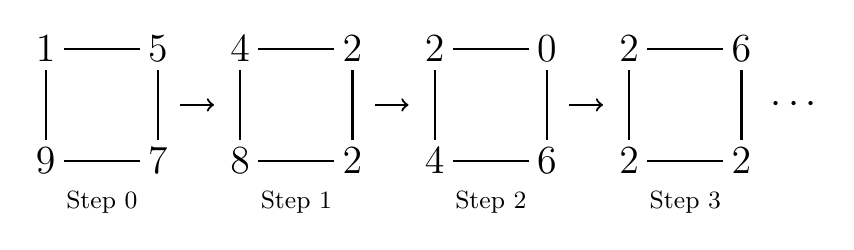
\begin{tikzpicture}[
    scale=0.95,
    number/.style={
        fill=white,
        inner sep=3pt,
        font=\Large
    }
]
% Numbers are listed clockwise from the top-left corner.
\foreach \x/\a/\b/\c/\d
    [count=\stepnumber from 0] in {
    0/1/5/7/9,
    2.6/4/2/2/8,
    5.2/2/0/6/4,
    7.8/2/6/2/2
}{
    \begin{scope}[shift={(\x,0)}]
        \draw[thick] (0,0) rectangle (1.5,1.5);

        \node[number] at (0,1.5)   {$\a$};
        \node[number] at (1.5,1.5) {$\b$};
        \node[number] at (1.5,0)   {$\c$};
        \node[number] at (0,0)     {$\d$};

        \node[font=\small] at (0.75,-0.55)
            {Step \stepnumber};
    \end{scope}
}

\foreach \x in {1.8,4.4,7.0}{
    \draw[->,thick] (\x,0.75) -- ++(0.45,0);
}

\node[font=\Large] at (10,0.75) {$\cdots$};
\end{tikzpicture}
\end{frame}


\subsection{Wrapping up}

\begin{frame}{Question of the Day}
\pause
  \begin{block}{Puzzle}
    Take the numbers $\{1,2,\dots,2026\}$.  What's the largest subset of them with the property that no number divides another number?
  \end{block}
\end{frame}

\begin{frame}{Final thoughts}
  \begin{block}{Reflection}
    \begin{itemize}
\pause
      \item Give an example of creativity in mathematics.
\pause
      \item Give an example of what you can do to help promote creativity.
    \end{itemize}
  \end{block}
\begin{center}
Submit your responses by \textbf{Tonight!}
\end{center}
\end{frame}


\end{document}


